\documentclass{article}
\usepackage{color}
\usepackage{listings}
\usepackage{graphicx}
\usepackage{subfig}
\usepackage{caption}
\usepackage{subcaption}
\usepackage{amsmath}
\usepackage{cite}
\usepackage{setspace,lipsum}% http://ctan.org/pkg/{setspace,lipsum}

\lstset{ %
language=java,                % choose the language of the code
basicstyle=\footnotesize,       % the size of the fonts that are used for the code
numbers=left,                   % where to put the line-numbers
numberstyle=\footnotesize,      % the size of the fonts that are used for the line-numbers
stepnumber=1,                   % the step between two line-numbers. If it is 1 each line will be numbered
numbersep=5pt,                  % how far the line-numbers are from the code
backgroundcolor=\color{white},  % choose the background color. You must add \usepackage{color}
showspaces=false,               % show spaces adding particular underscores
showstringspaces=false,         % underline spaces within strings
showtabs=false,                 % show tabs within strings adding particular underscores
frame=single,           % adds a frame around the code
tabsize=2,          % sets default tabsize to 2 spaces
captionpos=b,           % sets the caption-position to bottom
breaklines=true,        % sets automatic line breaking
breakatwhitespace=false,    % sets if automatic breaks should only happen at whitespace
escapeinside={\%*}{*}          % if you want to add a comment within your code
}

% Informationen ------------------------------------------------------------
% 	Definition von globalen Parametern, die im gesamten Dokument verwendet
% 	werden können (z.B auf dem Deckblatt etc.).
% --------------------------------------------------------------------------
\newcommand{\titel}{The Glorious Title of my Master/Bachlor Thesis/Exposé}
\newcommand{\art}{Exposé} %Bachelorarbeit
\newcommand{\ort}{Leipzig}
\newcommand{\hochschule}{Universität Leipzig}
\newcommand{\fachgebiet}{Abteilung Datenbanken}
\newcommand{\fakultaet}{Fakultät für Mathematik und Informatik}
\newcommand{\institut}{Institut für Informatik}
\newcommand{\autor}{xxxx xxxxx}
\newcommand{\matrikelnr}{xxxxxxx}
\newcommand{\erstbetreuer}{Prof. Dr. Erhard Rahm}
\newcommand{\zweitbetreuer}{XXXXX}
\newcommand{\jahr}{xxxx}
\newcommand{\invnr}{1337}
\newcommand{\eingereicht}{xx.xx.xxxx}

% Eigene Befehle
\newcommand{\todo}[1]{\textbf{\textsc{\textcolor{red}{(TODO: #1)}}}}

% Autorennamen in small caps
\newcommand{\AutorZ}[1]{\textsc{#1}}
\newcommand{\Autor}[1]{\AutorZ{\citeauthor{#1}}}

% Befehle zur semantischen Auszeichnung von Text
\newcommand{\NeuerBegriff}[1]{\textbf{#1}}
\newcommand{\Fachbegriff}[1]{\textit{#1}}
\newcommand{\Prozess}[1]{\textit{#1}}
\newcommand{\Webservice}[1]{\textit{#1}}
\newcommand{\Eingabe}[1]{\texttt{#1}}
\newcommand{\Code}[1]{\texttt{#1}}
\newcommand{\Datei}[1]{\texttt{#1}}
\newcommand{\Datentyp}[1]{\textsf{#1}}
\newcommand{\XMLElement}[1]{\textsf{#1}}

% Abkürzungen
\newcommand{\vgl}{Vgl.\ }
\newcommand{\ua}{\mbox{u.\,a.\ }}
\newcommand{\zB}{\mbox{z.\,B.\ }}
\newcommand{\bs}{$\backslash$}

% Einfache Anführungszeichen in texttt
\newcommand{\sq}{\textquotesingle}


\begin{document}

\thispagestyle{plain}
\begin{titlepage}

\begin{center}

\institut\\
\fakultaet\\
\fachgebiet\\[6ex]

\textbf{\large\titel}\\[1.5ex]
\art\\[6ex]

\normalsize
vorgelegt von:\\
\autor\\[1.5ex]
Matrikelnummer:\\
\matrikelnr\\[1.5ex]
Betreuer:\\
\erstbetreuer\\
\zweitbetreuer\\[1.0ex]
\end{center}

%\begin{tabbing}
%\hspace{3.5cm}\= \kill
%   vorgelegt von: \> \autor\\[1.2ex]
%   Matrikelnummer: \> \matrikelnr\\[1.2ex]
%    \> \\
%   Betreuer: \> \erstbetreuer\\[1.2ex]
%    \> \zweitbetreuer
%\end{tabbing}

\begin{center}
\copyright\ \jahr\\[1.0ex]
\end{center}

\singlespacing
\small
\noindent Dieses Werk einschließlich seiner Teile ist \textbf{urheberrechtlich geschützt}. Jede Verwertung außerhalb der engen Grenzen des Urheberrechtgesetzes ist ohne Zustimmung des Autors unzulässig und strafbar. Das gilt insbesondere für Vervielfältigungen, Übersetzungen, Mikroverfilmungen sowie die Einspeicherung und Verarbeitung in elektronischen Systemen.

\end{titlepage}


\tableofcontents{}

\newpage
\section{Einführung}
Die Performanz eines Rechners ist die Leistungsfähigkeit und Effizienz bei der Ausführung von Aufgaben. Um herauszufinden, welche ausgewählten Systeme die beste Performanz liefert, werden Benchmarks verwendet.  
Mit ihnen kann man die Rechenleistung oder auch Lese-/Schreibgeschwingkeit der Hardware oder auch Software mit standardisierten Tests messen \cite{benchmarkingBruno2014}. Ein Beispiel, bei dem Software getestet wird, sind virtuelle Maschinen.
Hier werden die Grenzen von virtuellen CPUs oder des Hypervisor analysiert \cite{9256518}.
Auch im Cloudcomputing Bereich wird Benchmarking betrieben, um auch Performanz zwischen verschieden Cloudplatformen vergleichen zu können \cite{10.1145/2493123.2462919}.  Somit gibt es ein weites Spektrum an Auswahl von Systemen, wo solche Benchmarks verwendet werden können, um Grenzen zu testen und zu vergleichen.
Solche Grenzen könnten die Hardware (z. B. CPU-Taktrate oder Brandbreitengeschwindigkeit beim Lesen oder Schreiben), aber auch Software (Virtuelle Maschinen) sein.
Und mit der Verbesserung von solchen Speichermedien, wie HDD zu SSD, und CPU-Leistung wird die I/O Geschwindigkeit immer relevanter. Studien haben schon bewiesen, dass dies eine Ursache für Bottlenecks in der Performanz ist \cite{analysisNVMeSSD}.

In Großkonzernen sind oft Performanzprobleme die eigentlichen Hindernisse, und nicht die funktionellen Probleme. Serviceausfälle sind höchst kostspielig und sollten minimiert werden. \cite{whenStopPerformanceTest}. 
Aus diesem Grund werden solche Benchmarks in Hochleistungsrechner (High Performance Computing - HPC) durchgeführt, um ihre Grenzen zu analysieren.
Ein Beispielprogramm für so ein Benchmark Tool ist das Fio (flexible I/O tester) \cite{axboe2021github}.
Fio ist ein Tool, mit dem man die Brandbreitengeschwindigkeit vom Lesen/Schreiben testen kann. Diese Tests lassen sich als eine Logdatei ausgeben.
Mein Programm wird mit diesen Logs arbeiten, um sie darstellen und analysieren zu können. Da diese Dateien zehntausende von Zeilen besitzen können.
In meiner Arbeit werde ich mit dem fio Tool arbeiten, um solche Performanceänderungen zu analysieren und den stationären Zustand zu ermitteln. Ein Zustand, wo die Rechenleistung oder Lese-/Schreibgeschwindigkeit sich nicht mehr beim Messen stark ändert \cite{vmsHotandCold}.

\section{Grundlagen}
Das Fio Tool ermöglicht das Testen auf bestimmter Hardware oder Software. Die I/O-Geschwindigkeit wird hier in Mebibyte pro Sekunde angegeben. Das Fio bietet auch die Möglichkeit diese Einheit zu ändern.
Das Programm selbst besitzt kein GUI, sondern arbeitet nur in der Konsole. Man kann für das Programm sogenannte .fio Dateien schreiben. Oder man arbeitet direkt in der Konsole,
um seine gewünschten Tests durchzuführen.
Wenn man nun ein Random Read testen möchte, kann die .fio Datei wie folgt aussehen (Listing \ref{lst:log_line_example}):
\newpage
\begin{lstlisting}[caption=Beispiel für eine .fio Datei,label={lst:fio_file_example}]
    ; fio-rand-read.job for fio Test

    [global]

    name=rand-read # Name des Jobs
    rw=randread # Was soll der Job testen, randread = random read
    runtime=2s # Wie lange soll der Job laufen
    size=128m # Groesse der Datei, m fuer Megabyte
    write_bw_log=mytest # Name der Log-Datei
\end{lstlisting}
\bigskip
In der Konsole kann man sie auch einzeln als Parameter angeben, wenn es nur ein Test sein soll.
Diese Tests, oder auch Jobs genannt, geben Logs aus, mit denen mein Tool arbeiten wird. Dieser Job oben testet das Random Read mit einer
Laufzeit (Runtime) von 2 Sekunden und liest eine Datei mit einer Größe von 128 Mebibyte. Mit größeren Tests ist es möglich, den stationären Zustand zu analysieren. 
Der stationäre Zustand ist der Zeitpunkt, wenn es keine starken Schwankungen mehr bei der Brandbreitengeschwindigkeit im Lesen oder im Schreiben gibt.
Ein Hindernis bei dieser Analyse könnten die nicht deterministischen Faktoren sein.
Auch wenn man das Lesen/Schreiben auf demselben System mit derselben Datei testet, ist die Brandbreitengeschwindigkeit im Durchschnitt nie die gleiche. Sie wird immer abweichen.
Ursachen dafür könnten schon verschiedene CPU-Temperaturen sein, aber auch CPU-Scaling oder parallele Prozessierung \cite{baseline}.
Das fio selbst arbeitet nicht nur mit einem Thread. Sondern es arbeitet mit Multithreads, was nicht deterministische Zustände hervorrufen kann.
Da die Geschwindigkeit sich nie konstant einem Wert nähert, sondern immer abweicht, soll mein Programm in Zukunft mithilfe der Standardabweichung den stationären Zustand ermitteln.
Solche Abweichung könnte in wenigen Prozentbereichen liegen. 

Es wird aber nicht ausreichen, ein paar Tests durchzuführen und danach die Logs davon auszuwerten. Diese Logs wären nämlich nicht akkurat genug.
Man muss erst einige Warm-up-Iterationen durchführen. Erst dann werden die Werte am Ende präziser \cite{vmsHotandCold}. Somit hängt der stationäre Zustand, der errechnet werden soll, 
mit diesen Warmups zusammen. Dieses Problem wird aber nur ein Hindernis sein. Ein größeres Problem wird es sein - wenn der Warmup durchgelaufen ist -
welche Logs die besten Informationen besitzen. 
Die Auswahl der Logs und deren Auswertung könnten signifikante Unterschiede beinhalten, die die Evaluierung verändern könnten \cite{whenStopPerformanceTest}.

\newpage
\section{Konzept}
Das fio Tool bekommt den Parameter $\text{--} write\_bw\_logs = [Dateiname]$ dazu, um die Logs als Datei auszugeben.
Diese Logs geben den kompletten Verlauf des Jobs wieder. Die ersten Zeilen des Logs könnten so aussehen, wie in Listing \ref{lst:log_line_example}:
\bigskip
\begin{lstlisting}[caption=Erste Zeilen des Logs (Bezeichnungen sind nicht im Log enthalten),label={lst:log_line_example}]
    [Time,	Bandwidth,  data direction, Blocksize,	Offset]
    0, 	  59782,        0,		          4096,		   0
    0, 	  54353,        0,		          4096,		   0
    1, 	  45545,        0,		          4096,		   0
\end{lstlisting}
\bigskip
Time für die Zeit in Millisekunden (ms) die verlaufen ist, Bandwidth für die Brandbreitengeschwindigkeit in Kibibyte/s, 
der dritte Wert für die data direction, ob gelesen (= 0) oder geschrieben (= 1) wurde und ein Blocksize
und ein Offset. Die Logdaten selbst sind immens lang und nicht schön lesbar. Deshalb wurde schon ein kleines Tool in Python programmiert,
was diese Logdaten zu einem Graph umwandelt. 
Das Tool nimmt die Zeit als X-Achse und die Brandbreitengeschwindigkeit als Y-Achse.
Wenn man sich die Logdaten als Text nochmal anschaut, sieht man, dass die Brandbreitengeschwindigkeit sich schneller innerhalb einer 1 ms ändert.
Das Python-Tool umgeht das Problem so, dass die Werte, die mehrfach doppelt vorkommen, linear auftrennt.
Unten wird es nochmal veranschaulicht (Listing \ref{lst:log_timesplit_example}), wenn die Zeit sich dreimal wiederholt, mit 23ms.
\bigskip
\begin{lstlisting}[caption={Aufsplitten der Zeit um ein Grafik zu bilden}, label={lst:log_timesplit_example}]
    Drei Zeilen aus der Logdatei
    [Time,	Bandwidth,	data direction, Blocksize,	Offset]
    23, 	    59782, 		0,		        4096,		0
    23, 	    43534, 		0,		        4096,		0
    23, 	    54364, 		0,		        4096,		0

    Erste beide Spalten     ->          X-Y-Koordinaten
    X: 23       Y: 59782    ->        X: 23.0     Y: 59782
    X: 23       Y: 43534    ->        X: 23.3     Y: 43534
    X: 23       Y: 54364    ->        X: 23.6     Y: 54364
\end{lstlisting}
\bigskip
In Figure \ref{fig:log_graphs}  ist einmal die Bandbreitengeschwindigkeit pro Millisekunde dargestellt (a) und in der anderen Abbildung (b) zeigt es die Häufigkeiten, 
wie oft diese Brandbreitengeschwindigkeit erreicht wurde. Das fio wurde wie oben in Listing \ref{lst:fio_file_example} ausgeführt.

\begin{figure}%
    \centering
    \subfloat[\centering Bandwidth Frequency]{{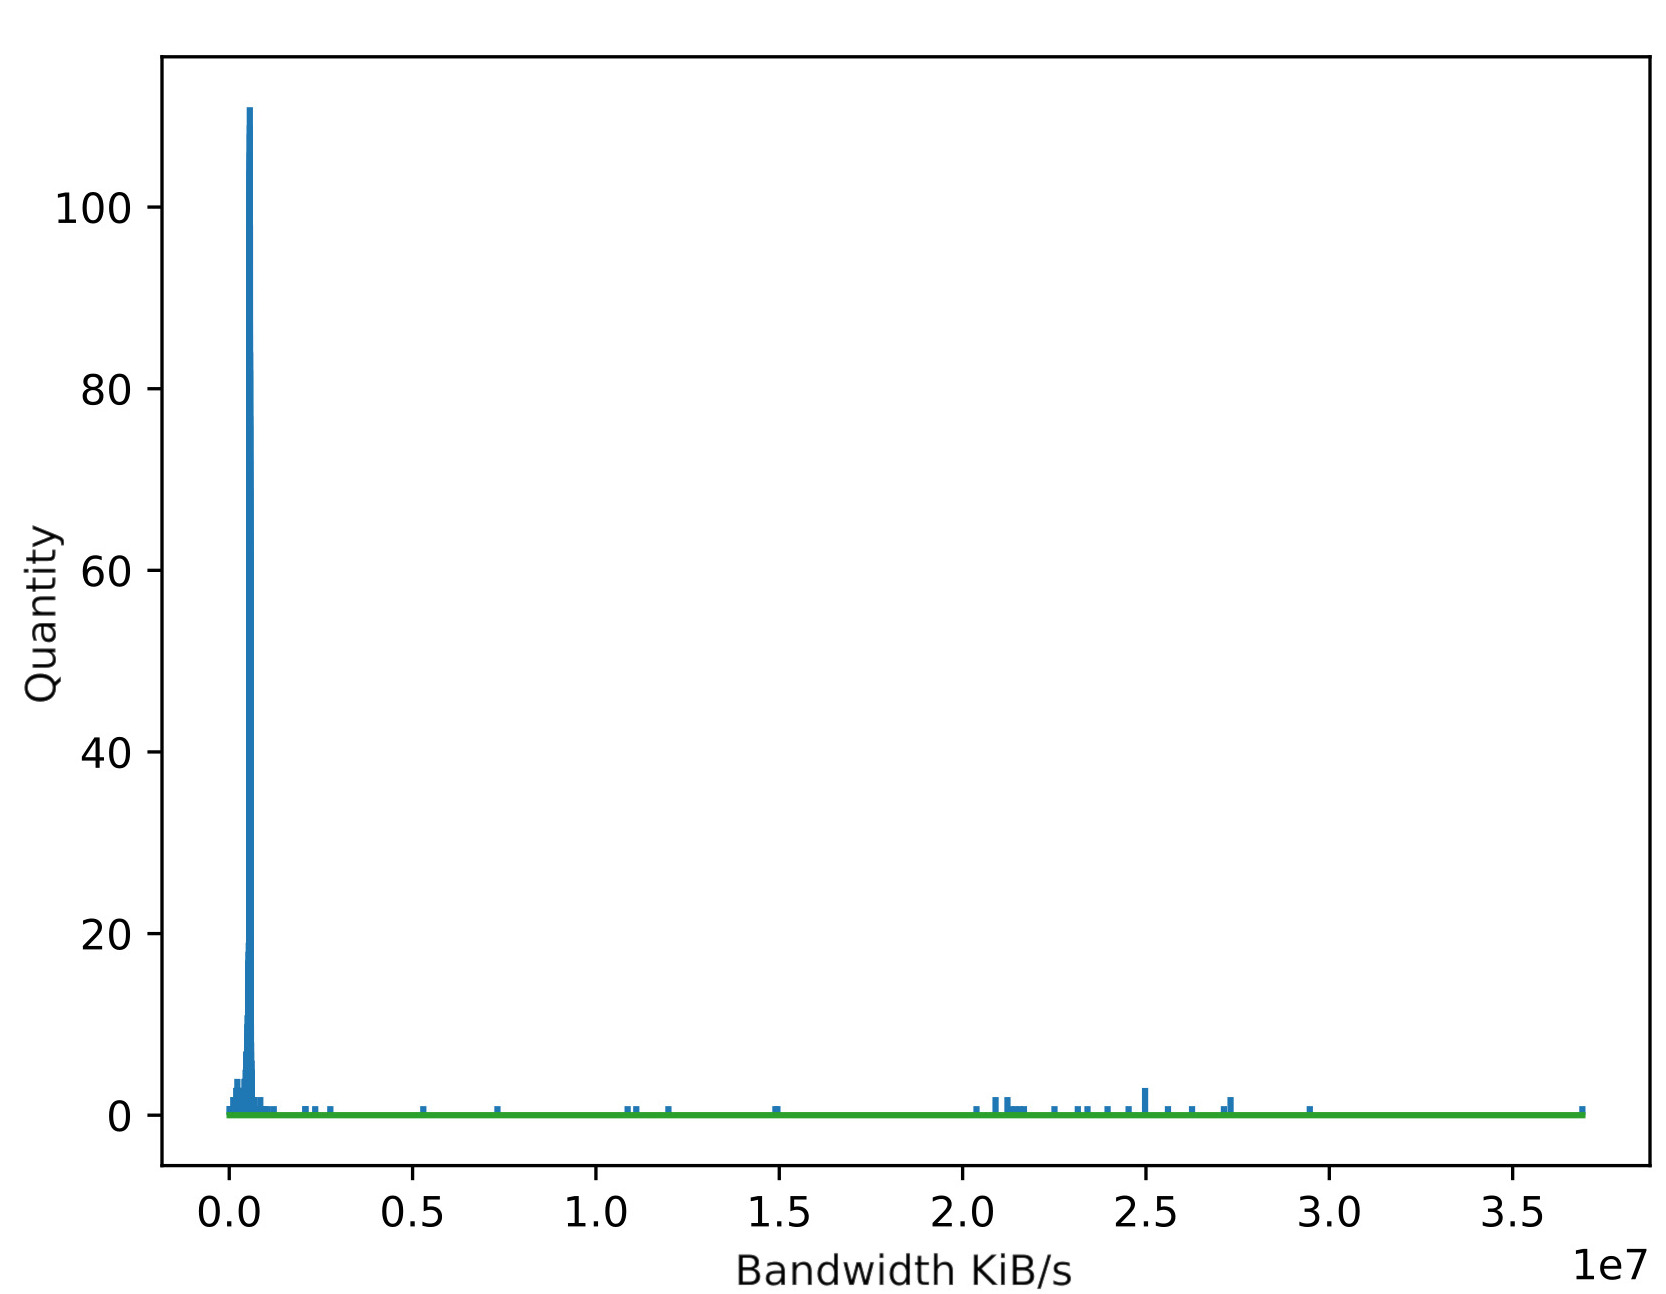
\includegraphics[width=5.5cm]{log_graph_bw_freq.jpg} }}%
    \qquad
    \subfloat[\centering Bandwidth per Msec]{{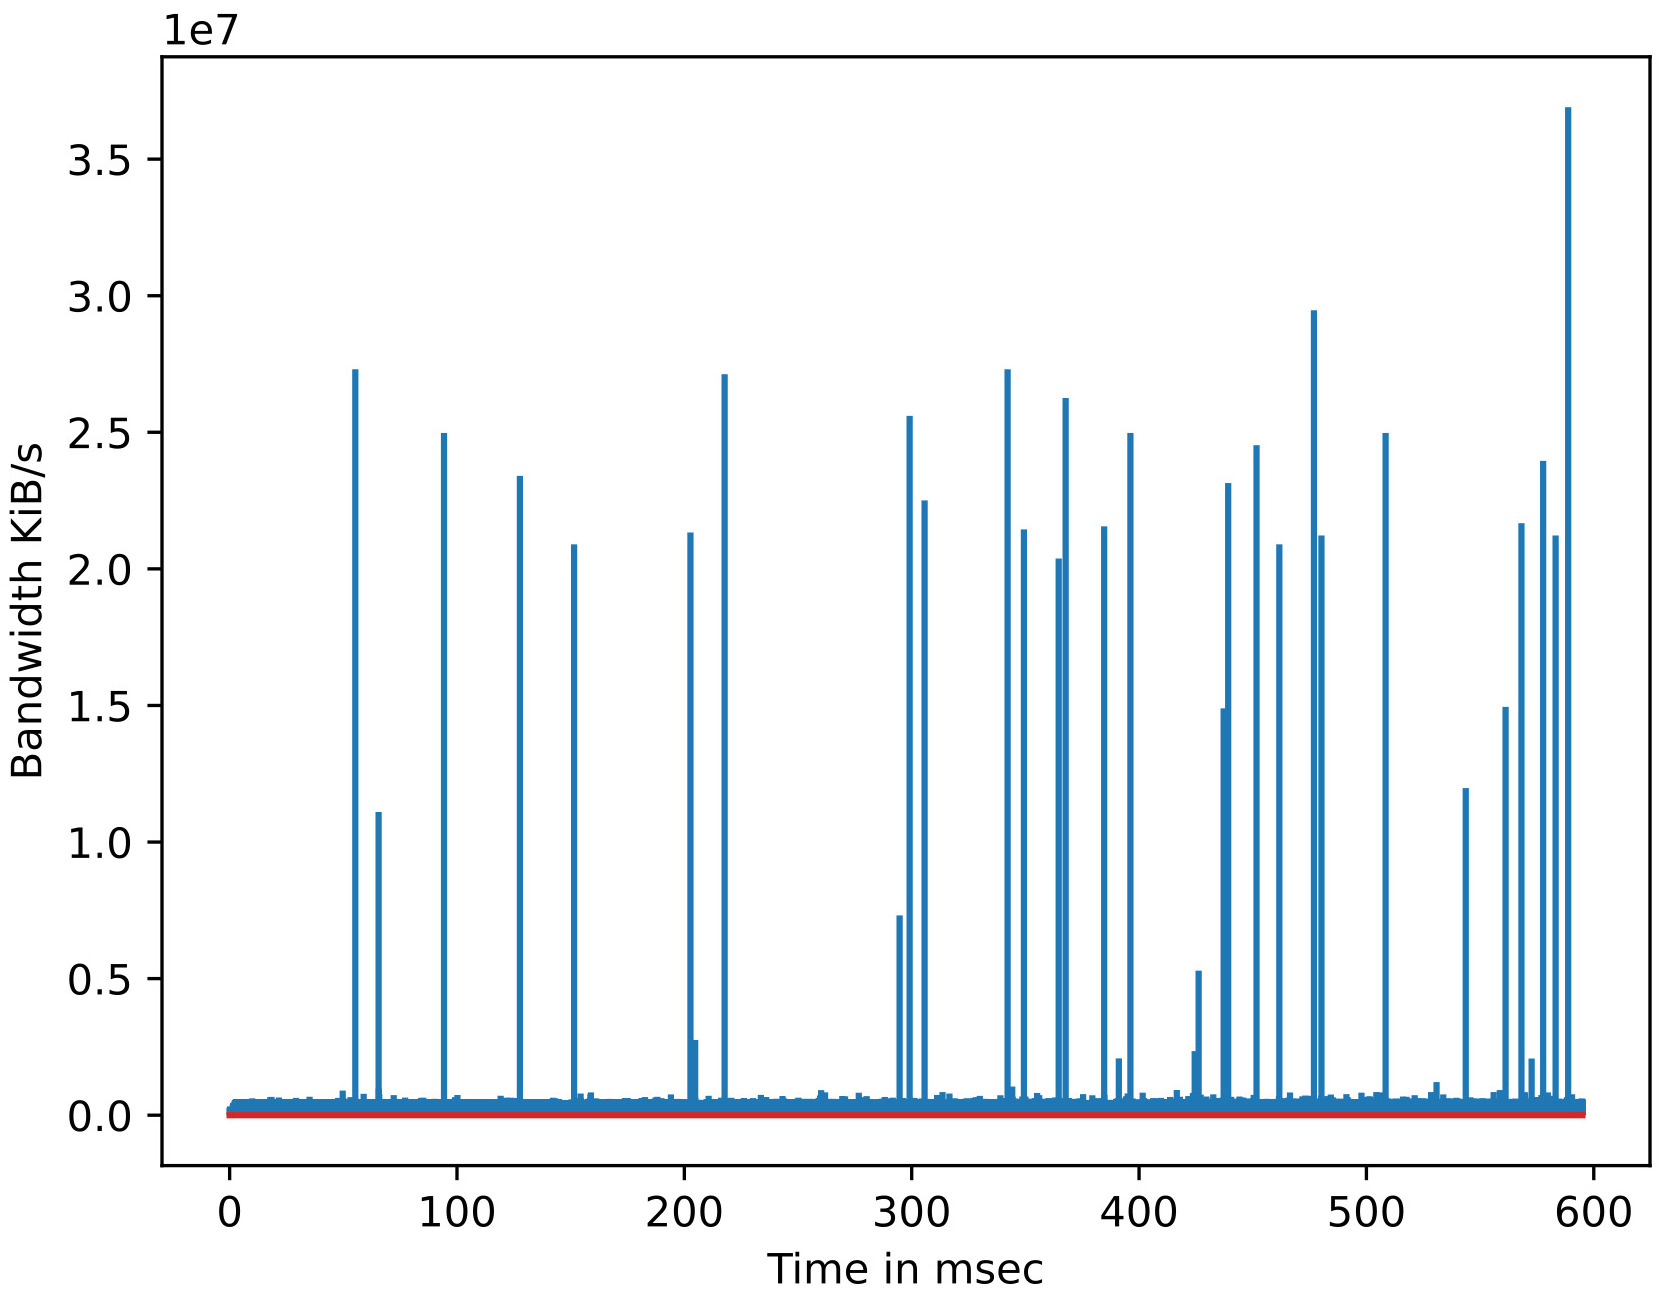
\includegraphics[width=5.5cm]{log_graph_time_to_bw.jpg} }}%
    \caption{fio Job: randread Bandbreite und Frequenz/Quantität}%
    \label{fig:log_graphs}%
\end{figure}


Der Computer, der verwendet wurde, hat ein 11th Gen Intel(R) Core(TM) i5-11400 @ 2.60GHz Prozessor und eine ADATA SWORDFISH 1TB SSD  als Datenträger.
Das kleine Tool diente mehr zum Einstieg. Die eigentliche Arbeit wird es sein, das Tool weiter auszubauen, das nicht nur veranschaulicht,
sondern auch den stationären Zustand berechnet.
Das Programm wird in Java geschrieben. Grund dafür ist, da dort bereits die meiste Erfahrung steckt.
Eine Möglichkeit, den stationären Zustand zu ermitteln, wäre, dass man die Standardabweichung verwendet und errechnet, wann die Abweichung klein genug ist und zusätzlich Konfidenzintervalle benutzt, um nicht determismus mitzubeachten.
Eine weitere Berechnung, die durchgeführt wird, ist die Verwendung der Varianz oder auch Varianzanalyse - \textit{Analysis of Variance} (ANOVA).
Da der stationare Zustand nicht eindeutig bestimmt werden kann, sollen diese statistischen Methoden dabei helfen.
ANOVA lässt sich mit dem Tukey HSD und t-Test erweitern, um signifikante Unterschiede bei paarweisen Messungen beim Testen zu analysieren. So soll mein Tool mit den Logdateien statistisch arbeiten.

\section{Verwandte Arbeiten}
In der Arbeit von Barrett et al. wurde tiefer in nicht Determinismus von VMs eingegangen.
Dort wurde versucht, nicht determinisitsche Faktoren so gering wie möglich zu halten, da sonst Warmups nicht erfolgen können, auch wenn gleiche Workloads wiederholt durchlaufen werden. Und etwas andere Hardware und Operationssysteme haben wenig Einfluss auf die Zeit von Warmups. Li et al. arbeiteten ebenfalls mit VMs und testen die Performanz von diesen Maschinen mit verschiedener Anzahl an virtuellen CPUs. Und eine große Anzahl an VCPUs erhöht nicht zwingend die Performanz.
Georges et al. verwendet statistische Methoden, wie Varianzanalyse und Tukey HSD, um eine akkurate Auswertung von den Experimenten berechnen zu können. Sie arbeiten ebenfalls mit VMs und VM Warmups.
Gründe für nicht deterministisches Verhalten in VMs könnte Garbage Collection, Thread Scheduling oder auch Just-in-Time Compilation/Optimization sein (Arbeit von Georg Reichelt et al.).
AlGhmadi et al. erarbeiteten, wann Performanztests nach langem Testen redundant werden und wie viele Tests genug sind.
 
\newpage
\section{Zeitplan}
- - 
\bibliography{cite}{}
\bibliographystyle{plain}
\end{document}